\section{Introduction}
\label{sec:introduction}

% state the learning objective 

\hspace{0,5cm} This report is being made for the subject of Circuit Theory and Electronics Fundamentals and is related to the $1^{st}$ laboratory.

The objective of this laboratory assignment is to study a circuit containing seven resistors, one voltage source, one current source, one current controlled voltage source and one voltage controlled current source. The elementary meshes are named after the current to which they are attributed and so there are four of them.

The current controlled voltage source Vc is calculated by multiplying Kc with the current Ic, whereas the voltage controlled current source Ib can be determined by multiplying Kb with the voltage source Vb.

The display of this circuit can be seen in Figure~\ref{fig:circuito}.

In Section~\ref{sec:analysis} we will analise theorically the circuit by both Method Analysis and present the results obtained by Octave.

Secondly, in Section~\ref{sec:simulation} we will simulate the circuit using ngspice, present the results obtained and compare them with the ones gathered from Section~\ref{sec:analysis}.

The conclusions of this study are outlined in Section~\ref{sec:conclusion}.

\begin{figure}[h] \centering
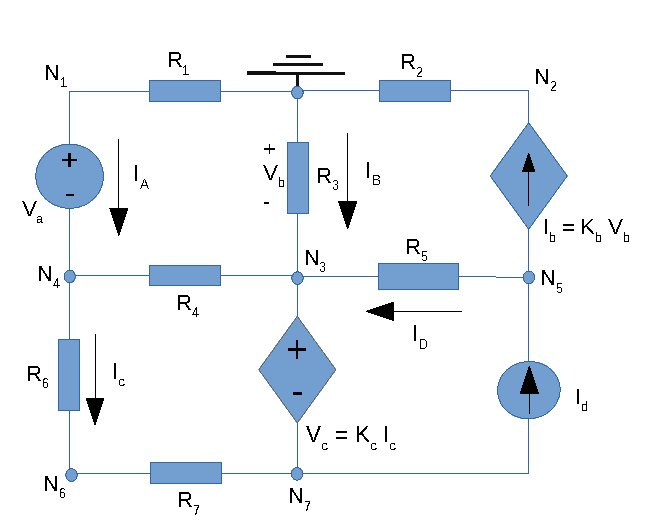
\includegraphics[width=0.7\linewidth]{circuito.pdf}
\caption{Circuit with the nodes} %mudar legendaaaaaaaaaaa!!!!!!
\label{fig:circuito}
\end{figure}


\begin{center}
Where:

$R_1 = 1.03431507833 $

$R_2 = 2.02853090731$
 
$R_3 = 3.1462050633 $

$R_4 = 4.03438547455$ 

$R_5 = 3.12170042214 $

$R_6 = 2.07116379646 $

$R_7 = 1.01597753093 $

$V_a = 5.156959346 $

$I_d = 1.01455683569 $

$K_b = 7.1497941196 $

$K_c = 8.12593642585 $
\end{center}

The units of the elements whose name starts with R (the resistors) are kOhm (kiloohm), the ones that start with I are expressed in mA (miliampere) and the ones starting with V are expressed in V (volts). While Kb is given in mS (milisiemens), Kc is also given in kOhm.

These values where obtained using the \textit{Python} script using the lowest student number on our group - 95785.


